\section{Netzarchitektur}
\label{raeumliche_netzarchitektur}

% Hier den Cube vorstellen
% 1D Convolutions etc

\begin{figure}[t]
\centering
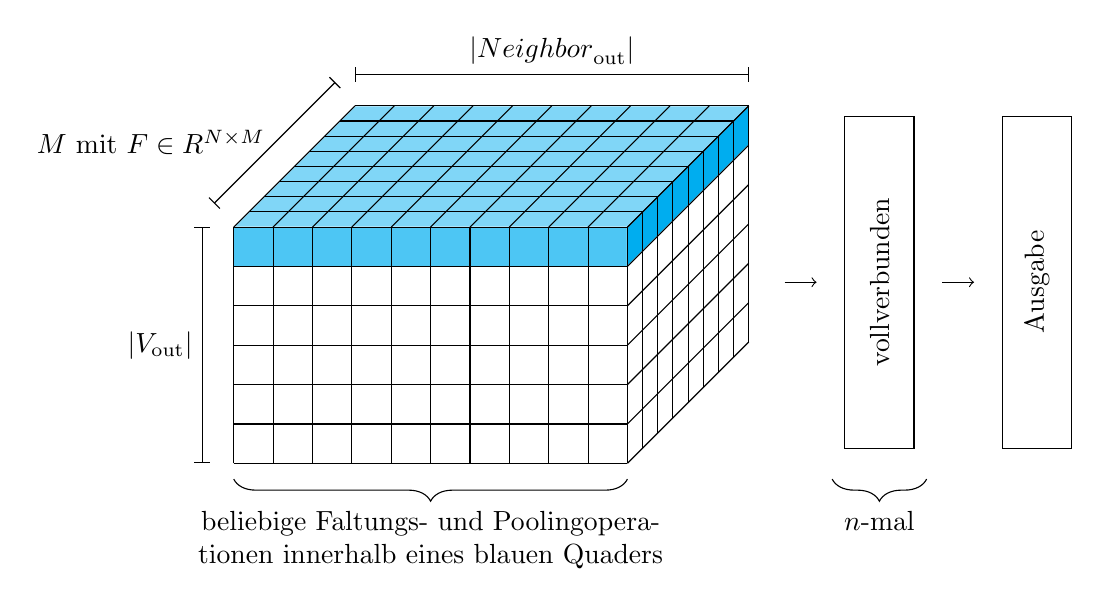
\begin{tikzpicture}
  \draw[white,fill=cyan!70] (0, 3, 4) -- (5, 3, 4) -- (5, 2.5, 4) -- (0, 2.5, 4) -- cycle;
  \draw[white,fill=cyan!50] (0, 3, 4) -- (5, 3, 4) -- (5, 3,   0) -- (0, 3,   0) -- cycle;
  \draw[white,fill=cyan]    (5, 3, 4) -- (5, 3, 0) -- (5, 2.5, 0) -- (5, 2.5, 4) -- cycle;
  \tikzstyle{path}=[->, shorten >= 10pt, shorten <= 10pt]
  \tikzstyle{node}=[rectangle,draw, minimum width=120pt, minimum height=25pt, inner sep=0pt, fill=white, rotate=90]
  \tikzstyle{noborder}=[draw=none,fill=none]

  \foreach \x in {0,0.5,1,1.5,2,2.5,3} {%
    \draw (0,  \x, 4)  -- (5,  \x, 4);
    \draw (5,  \x, 4)  -- (5,  \x, 0);
  }
  \foreach \x in {0,0.5,1,1.5,2,2.5,3,3.5,4,4.5,5} {%
    \draw (\x, 0,  4)  -- (\x, 3,  4);
    \draw (\x, 3,  4)  -- (\x, 3,  0);
  }
  \foreach \x in {0,0.5,1,1.5,2,2.5,3,3.5,4} {%
    \draw (5,  0,  \x) -- (5,  3, \x);
    \draw (0,  3,  \x) -- (5,  3, \x);
  }

  \draw[|-|] (-0.4, 0,    4)    -- node[left]  {$\left|\gls{V}_{\mathrm{out}}\right|$}        (-0.4, 3,    4);
  \draw[|-|] (0,    3.55, 4.65) -- node[left]  {$M$ mit $\ma{F} \in \gls{R}^{N \times M}$}    (0,    3.55, 0.65);
  \draw[|-|] (0,    3.4,  0)    -- node[above] {$\left|\gls{Neighbor}_{\mathrm{out}}\right|$} (5,    3.4,  0);

  \node[node, noborder] (0) at (6.2,  2.3, 4) {};
  \node[node]           (1) at (8.2,  2.3, 4) {vollverbunden};
  \node[node]           (2) at (10.2, 2.3, 4) {Ausgabe};

  \path[path] (0) edge (1);
  \path[path] (1) edge (2);

  \draw [decoration={brace,mirror,amplitude=8pt},decorate,-] (0,-0.2,4) -- node[below=8pt,text width=8cm, align=center] {beliebige Faltungs- und Poolingoperationen innerhalb eines blauen Quaders} (5,-0.2,4);
  \draw [decoration={brace,mirror,amplitude=8pt},decorate,-] (7.6,-0.2,4) -- node[below=8pt] {$n$-mal} (8.8,-0.2,4);

\end{tikzpicture}
\caption[Räumliche Netzarchitektur auf Graphen]{Typische räumliche Netzarchitektur auf Graphen.
Der \emph{Quader}, der durch die Anordnung der Knoten entsprechend ihrer Nachbarschaften entsteht, kann entlang der Nachbarschaften und ihrer Merkmale beliebig oft gefaltet und gepoolt werden.
Eine Faltung entlang der Knotenauswahl besitzt allerdings keine Bedeutung und ist deshalb zu vermeiden.
Im Anschluss können vollverbundene Schichten hin zur Ausgabe an den abgeflachten Quader gestapelt werden.}
\label{fig:netzarchitektur_raeumlich}
\end{figure}


Eigentliche Graphstruktur geht verloren (\zB{} Distanzen der Knoten zueinander) (in gewisser weise stecken diese aber in den Formfeatures).

Die Anordnung der Knoten zu einem Quaderform besitzt damit die Einschränkung, dass das Netz lediglich eine Faltungsschicht enthalten kann.
Die Methode der spektralen Faltung auf Graphen umgeht diese Einschränkung.

Würfel ist speicherineffizient
